
\subsection{Configurazione Database}
Si è optato per l'utilizzo di ClickHouse per il salvataggio dei dati, le motivazioni sono descritte nella sezione \ref{sec:clickHouse}. In particolare, per ogni sensore dei quali si desidera memorizzare i dati, viene creata una tabella che acquisisce i dati dal relativo topic Kafka.
Le tipologie di sensori cui misurazioni si vogliono trattare nel progetto sono:
\begin{itemize}
    \item Sensori di temperatura;
    \item Sensori di umidità;
    \item Sensori di rilevamento polveri sottili; 
    \item Sensori stato riempimento isole ecologiche;
    \item Sensori di stato occupazione colonnine di ricarica;
    \item Sensori di guasti elettrici;
    \item Sensori del livello dell'acqua.
\end{itemize}

La configurazione del database ClickHouse è stata cruciale nella progettazione, poiché un'adeguata ottimizzazione consente di garantire prestazioni ottimali per un sistema orientato al tempo reale e in grado di gestire analisi su enormi volumi di dati.


\subsubsection{Funzionalità Clickhouse utilizzate}
\paragraph{Materialized Views}
Le Materialized Views in ClickHouse sono un meccanismo potente per migliorare le prestazioni delle query e semplificare l'accesso ai dati. Funzionano mantenendo una copia fisica dei risultati di una query di selezione, che viene quindi memorizzata su disco. Questa copia è aggiornata periodicamente in base ai dati sottostanti.

\paragraph*{Utilizzi Principali delle Materialized Views}
\begin{itemize}
    \item \textbf{Calcolo aggregazioni e popolamento tabelle}:Spesso le delle materialized Views sono state utilizzate per calcolare aggregazioni su dati e quindi popolare altre tabelle con i risultati aggregati. Ad esempio, nel caso specifico in cui una Materialized View calcola la media delle temperature per ogni sensore ogni secondo, i risultati di questa vista possono essere utilizzati per popolare una tabella principale contenente i dati di temperatura aggregati, aggiornando i valori di temperatura medi per ogni sensore ogni secondo;
    \item \textbf{Ottimizzazione delle Prestazioni}: memorizzando i risultati di una query complessa, le Materialized Views consentono di eseguire rapidamente le Query successive senza dover ricalcolare i dati ogni volta. Ciò è particolarmente utile in applicazioni che richiedono interrogazioni frequenti su grandi volumi di dati;
    \item \textbf{Decomposizione delle \textit{Query} Complesse}: le Materialized Views consentono di decomporre query complesse in passaggi più semplici e riutilizzabili, migliorando la leggibilità del codice e semplificando lo sviluppo e la manutenzione delle query.
\end{itemize}



\paragraph{MergeTree}\label{sec:MergeTree}
Link alla documentazione: \href{https://clickhouse.com/docs/en/engines/table-engines/mergetree-family/mergetree#mergetree}{ClickHouse - MergeTree}.\newline
MergeTree è uno dei motori di tabella più potenti e utilizzati in ClickHouse, noto per la sua capacità di gestire e memorizzare grandi volumi di dati in modo efficiente. È una scelta ideale per applicazioni che richiedono l'archiviazione e l'analisi di dati cronologicamente ordinati, come i dati di log o di monitoraggio. L'architettura di MergeTree organizza i dati in parti, ciascuna contenente una serie di punti dati ordinati cronologicamente. Questa organizzazione ottimizzata consente di eseguire rapidamente le query che richiedono l'accesso a dati specifici all'interno di un intervallo di tempo definito, garantendo prestazioni elevate anche su grandi dataset. Oltre alla gestione efficiente dei dati, MergeTree supporta funzionalità avanzate come la compressione dei dati e la gestione automatica delle partizioni. Queste caratteristiche consentono di ottimizzare ulteriormente le prestazioni e la gestione complessiva dei dati, rendendo MergeTree una scelta affidabile per una vasta gamma di scenari di utilizzo in ClickHouse.



\paragraph{Time To Live in ClickHouse} \label{sec:RollupTTL}
Link alla documentazione: \href{https://clickhouse.com/docs/en/guides/developer/ttl#implementing-a-rollup}{ClickHouse - Implementing a Rollup}\newline
In ClickHouse, la funzionalità TTL (Time To Live) è un elemento chiave per gestire grandi volumi di dati in modo efficiente e garantire la pulizia automatica di informazioni obsolete o non più rilevanti. \\
Quando si specifica il motore Rollup per definire una tabella in ClickHouse, si abilita la creazione di tabelle che supportano il TTL. Questo consente di impostare un periodo temporale dopo il quale i dati saranno eliminati automaticamente dalla tabella. La struttura a Rollup organizza i dati in parti, ciascuna contenente una serie di punti dati ordinati cronologicamente. Il TTL può essere configurato per ciascuna parte dei dati, offrendo un controllo preciso sulla conservazione delle informazioni nel tempo. Questa flessibilità è particolarmente utile per applicazioni che richiedono la conservazione di dati storici per un periodo limitato, come ad esempio i dati di log o di monitoraggio. \newline
Un esempio di come potrebbe può venire utilizzato il motore Rollup per il TTL in ClickHouse è il seguente:
\begin{verbatim}
    TTL toDateTime(timestamp) + INTERVAL 1 MONTH
\end{verbatim}
L'uso del TTL di tipo Rollup in questo contesto è cruciale per garantire che la tabella rimanga efficiente e gestibile nel tempo, eliminando automaticamente i dati più vecchi e non più necessari dopo un periodo di tempo specificato. Questo aiuta a ottimizzare le prestazioni complessive del sistema e a gestire in modo efficiente i grandi volumi di dati accumulati nel tempo.


\paragraph{Partition}\label{sec:Partition}
Link alla documentazione: \href{https://clickhouse.com/docs/en/engines/table-engines/mergetree-family/mergetree#partition-by}{ClickHouse - Partitioning}.\\
Le partizioni sono una funzionalità fondamentale di ClickHouse che consente di organizzare in modo efficiente e gestire grandi volumi di dati. Questa caratteristica permette di suddividere i dati in gruppi logici in base a criteri specifici, come il valore di una colonna o un intervallo di tempo. Grazie a questa organizzazione ottimizzata, le query che richiedono l'accesso a dati specifici all'interno di una partizione possono essere eseguite rapidamente, garantendo prestazioni elevate anche su dataset di grandi dimensioni.\\
L'utilizzo delle partizioni nel nostro contesto viene giustificato dall'utilizzo di un TTL (Time To Live), infatti l'utilizzo combinato di queste due funzionalità consente:
\begin{itemize}
    \item Una gestione efficace dei dati nel tempo;
    \item Migliori prestazioni del sistema;
    \item Una semplificazione nella manutenzione del database.
\end{itemize}
Il partizionamento basato sul timestamp è una pratica comune in ClickHouse, poiché consente di organizzare i dati in partizioni in base al periodo temporale, ad esempio mensilmente. Questo approccio ottimizza l'archiviazione e facilita l'analisi dei dati di serie temporali, come le temperature o i log di eventi. Grazie a questa struttura, le query che coinvolgono dati all'interno di specifici intervalli temporali diventano più efficienti, consentendo un accesso rapido e una migliore analisi dei dati.




    
\paragraph{Projection}\label{sec:projections}
Link alla documentazione: \href{https://clickhouse.com/docs/en/sql-reference/statements/alter/projection}{https://clickhouse.com/docs/en/sql-reference/statements/alter/projection}\newline
Le proiezioni memorizzano i dati in un formato che ottimizza l'esecuzione delle \textit{Query}, questa caratteristica è utile per:

\begin{itemize}
    \item Eseguire \textit{Query} su una colonna che non fa parte della chiave primaria;
    \item Pre-aggregare colonne, riducendo sia i calcoli che l'I/O.
\end{itemize}

Puoi definire una o più proiezioni per una tabella e durante l'analisi della \textit{Query} la proiezione con meno dati da esaminare sarà selezionata da ClickHouse senza modificare la \textit{Query} fornita dall'utente.
\\
In generale l'introduzione delle PROJECTIONS produce risultati di notevole importanza, come illustrato di seguito. Consideriamo una tipica query eseguita per l'analisi tramite Grafana:
    
    \begin{lstlisting}[caption={Query tipica - Grafana}, captionpos=b]
      SELECT ID_sensore, avgMerge(value) AS value, timestamp
      FROM innovacity.temperatures
      WHERE (cella IN ('Arcella')) AND ((timestamp >= toDateTime64(1708338633507 / 1000, 3)) AND (timestamp <= toDateTime64(1708338933507 / 1000, 3) + INTERVAL 1 DAY))
      GROUP BY timestamp, ID_sensore
      HAVING (value >= -100) AND (value <= 100)

      --Query id: 48635435-9b35-4727-b580-9e33a9db92d4
    \end{lstlisting}

    \begin{figure}[H]
        \centering
        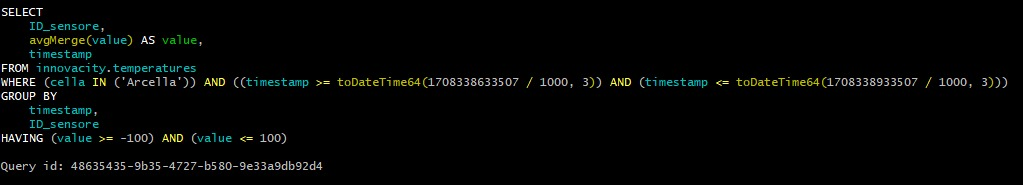
\includegraphics[width=1\textwidth]{../Images/SpecificaTecnica/ProjectionQuery.jpg}
        \caption{Query tipica - Grafana}
        \label{fig:ProjectionsQuery}
      \end{figure}
      Senza l'utilizzo delle PROJECTIONS, il risultato ottenuto è il seguente:
    \begin{figure}[H]
        \centering
        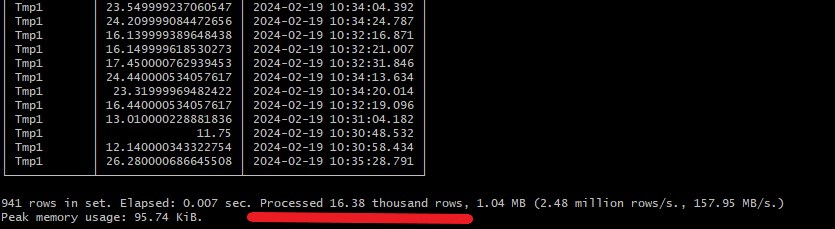
\includegraphics[width=0.9\textwidth]{../Images/SpecificaTecnica/SenzaProectionResult.jpg}
        \caption{Query tipica risultato senza projections}
        \label{fig:ProjectionsQueryWthout}
      \end{figure}
      ovvero sono state processate per ottenere il risultato della query \textbf{16,38} migliaia di righe. Invece in seguito all’aggiunta delle PROJECTIONS:

      \begin{figure}[H]
        \centering
        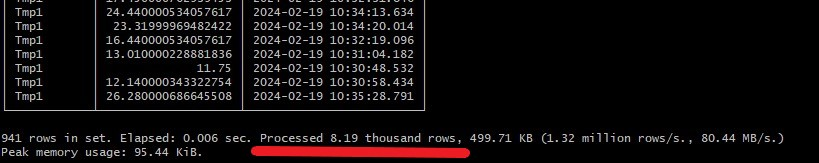
\includegraphics[width=0.9\textwidth]{../Images/SpecificaTecnica/ConProjectionRisultato.jpg}
        \caption{Query tipica risultato con projections}
        \label{fig:ProjectionsQueryWith}
      \end{figure}   
  Sono state elaborate approssimativamente 8,19 migliaia di righe per ottenere il risultato della query, circa la metà rispetto al conteggio precedente, evidenziando un miglioramento significativo. Inoltre, mediante un'interrogazione specifica è possibile confermare che le PROJECTIONS sono state effettivamente impiegate per generare il risultato della query in questione.
\begin{figure}[H]
    \centering
    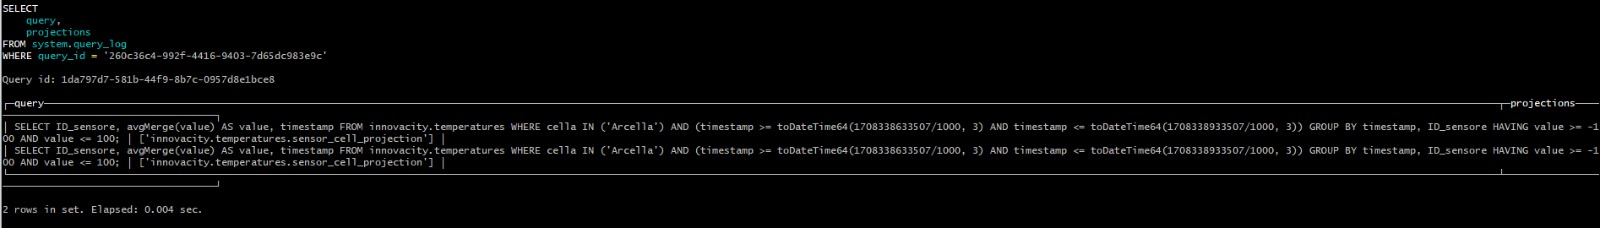
\includegraphics[width=1\textwidth]{../Images/SpecificaTecnica/ProjectionUsedByClickHouse.jpg}
    \caption{Uso della Projection}
    \label{fig:ProjectionsUsed}
\end{figure}

Considerando un'altra query eseguita dall'applicativo, che calcola la media globale di \textbf{170.000} misurazioni di temperatura, è possibile riconoscere i benefici derivanti dall'utilizzo delle PROJECTIONS. Alla conclusione dell'analisi, è evidente anche il loro effettivo impiego nel calcolo del risultato. Grazie all'adozione delle PROJECTIONS, si ottiene:
\begin{figure}[H]
    \centering
    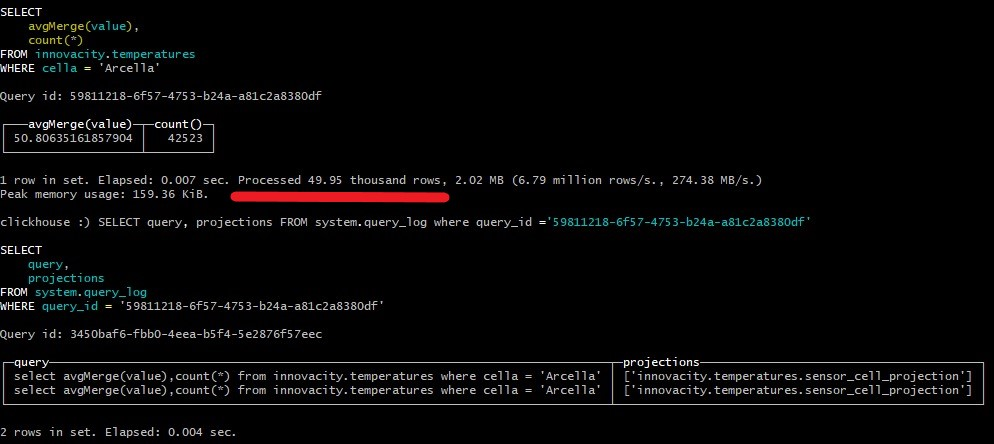
\includegraphics[width=1\textwidth]{../Images/SpecificaTecnica/query2ProjectionsWith.jpg}
    \caption{Query esempio Projection 2 - ClickHouse}
    \label{fig:with2proj}
  \end{figure}
Ovvero il totale di righe processate per ottenere il risultato è di \textbf{49,95 migliaia} con \textbf{0,07 secondi} di tempo utilizzati.
Si puo notare invece la differenza delle righe processate una volta rimossa la \textit{PROJECTIONS}:
\begin{figure}[H]
    \centering
    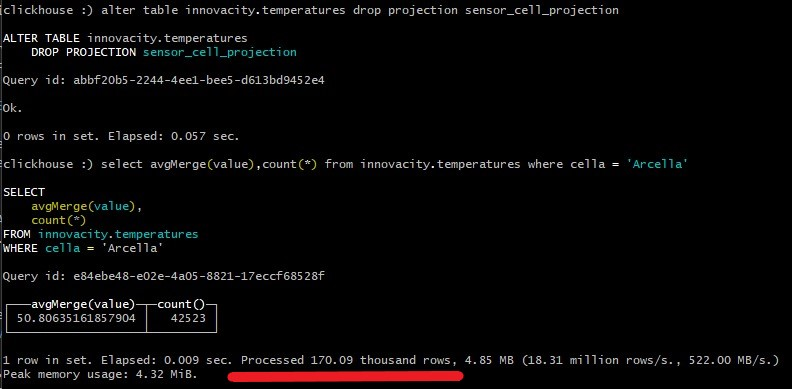
\includegraphics[width=1\textwidth]{../Images/SpecificaTecnica/query2ProjectionsWithout.jpg}
    \caption{Query esempio senza Projection 2 - ClickHouse}
    \label{fig:without2proj}
  \end{figure}

 Il totale di righe processate per ottenere il risultato è ora di \textbf{170,09 migliaia}, ovvero la totalità delle righe presenti nella tabella, con \textbf{0,09 secondi} di tempo utilizzati.

\paragraph*{Utilizzo dello spazio su disco}
\textbf{Attenzione:} le proiezioni creeranno internamente una nuova tabella nascosta, ciò significa che saranno necessari più I/O e spazio su disco. Ad esempio, se la proiezione ha definito una chiave primaria diversa, tutti i dati dalla tabella originale verranno duplicati.

\subsubsection{Integrazione tramite Kafka Engine in ClickHouse}\label{sec:kafka_engine}
ClickHouse supporta l'integrazione con Kafka tramite Kafka Engine, permettendo la lettura dei dati da un topic Kafka e il loro salvataggio in una tabella ClickHouse. Tale funzionalità riveste un'importanza notevole per applicazioni che richiedono l'elaborazione in tempo reale di dati provenienti da fonti esterne, una necessità frequente nel contesto del monitoraggio urbano. L'integrazione con Kafka consente l'acquisizione e la memorizzazione efficiente dei dati, garantendo prestazioni elevate anche su grandi volumi di dati.\\
Kafka Engine è progettato per il recupero di dati una sola volta. Ciò significa che una volta che i dati vengono interrogati da una tabella Kafka, vengono considerati consumati dalla coda. Pertanto, non si dovrebbero mai selezionare dati direttamente da una tabella di Kafka Engine, ma utilizzare invece una vista materializzata. Una vista materializzata viene attivata una volta che i dati sono disponibili in una tabella di Kafka Engine. Automaticamente sposta i dati da una tabella Kafka a una tabella di tipo MergeTree o Distributed. Quindi, sono necessarie almeno 3 tabelle:
\begin{itemize}
  \item La tabella di origine del motore Kafka;
  \item La tabella di destinazione (famiglia MergeTree o distribuita);
  \item Vista materializzata per spostare i dati;
\end{itemize}
\begin{figure}[H]
  \centering
  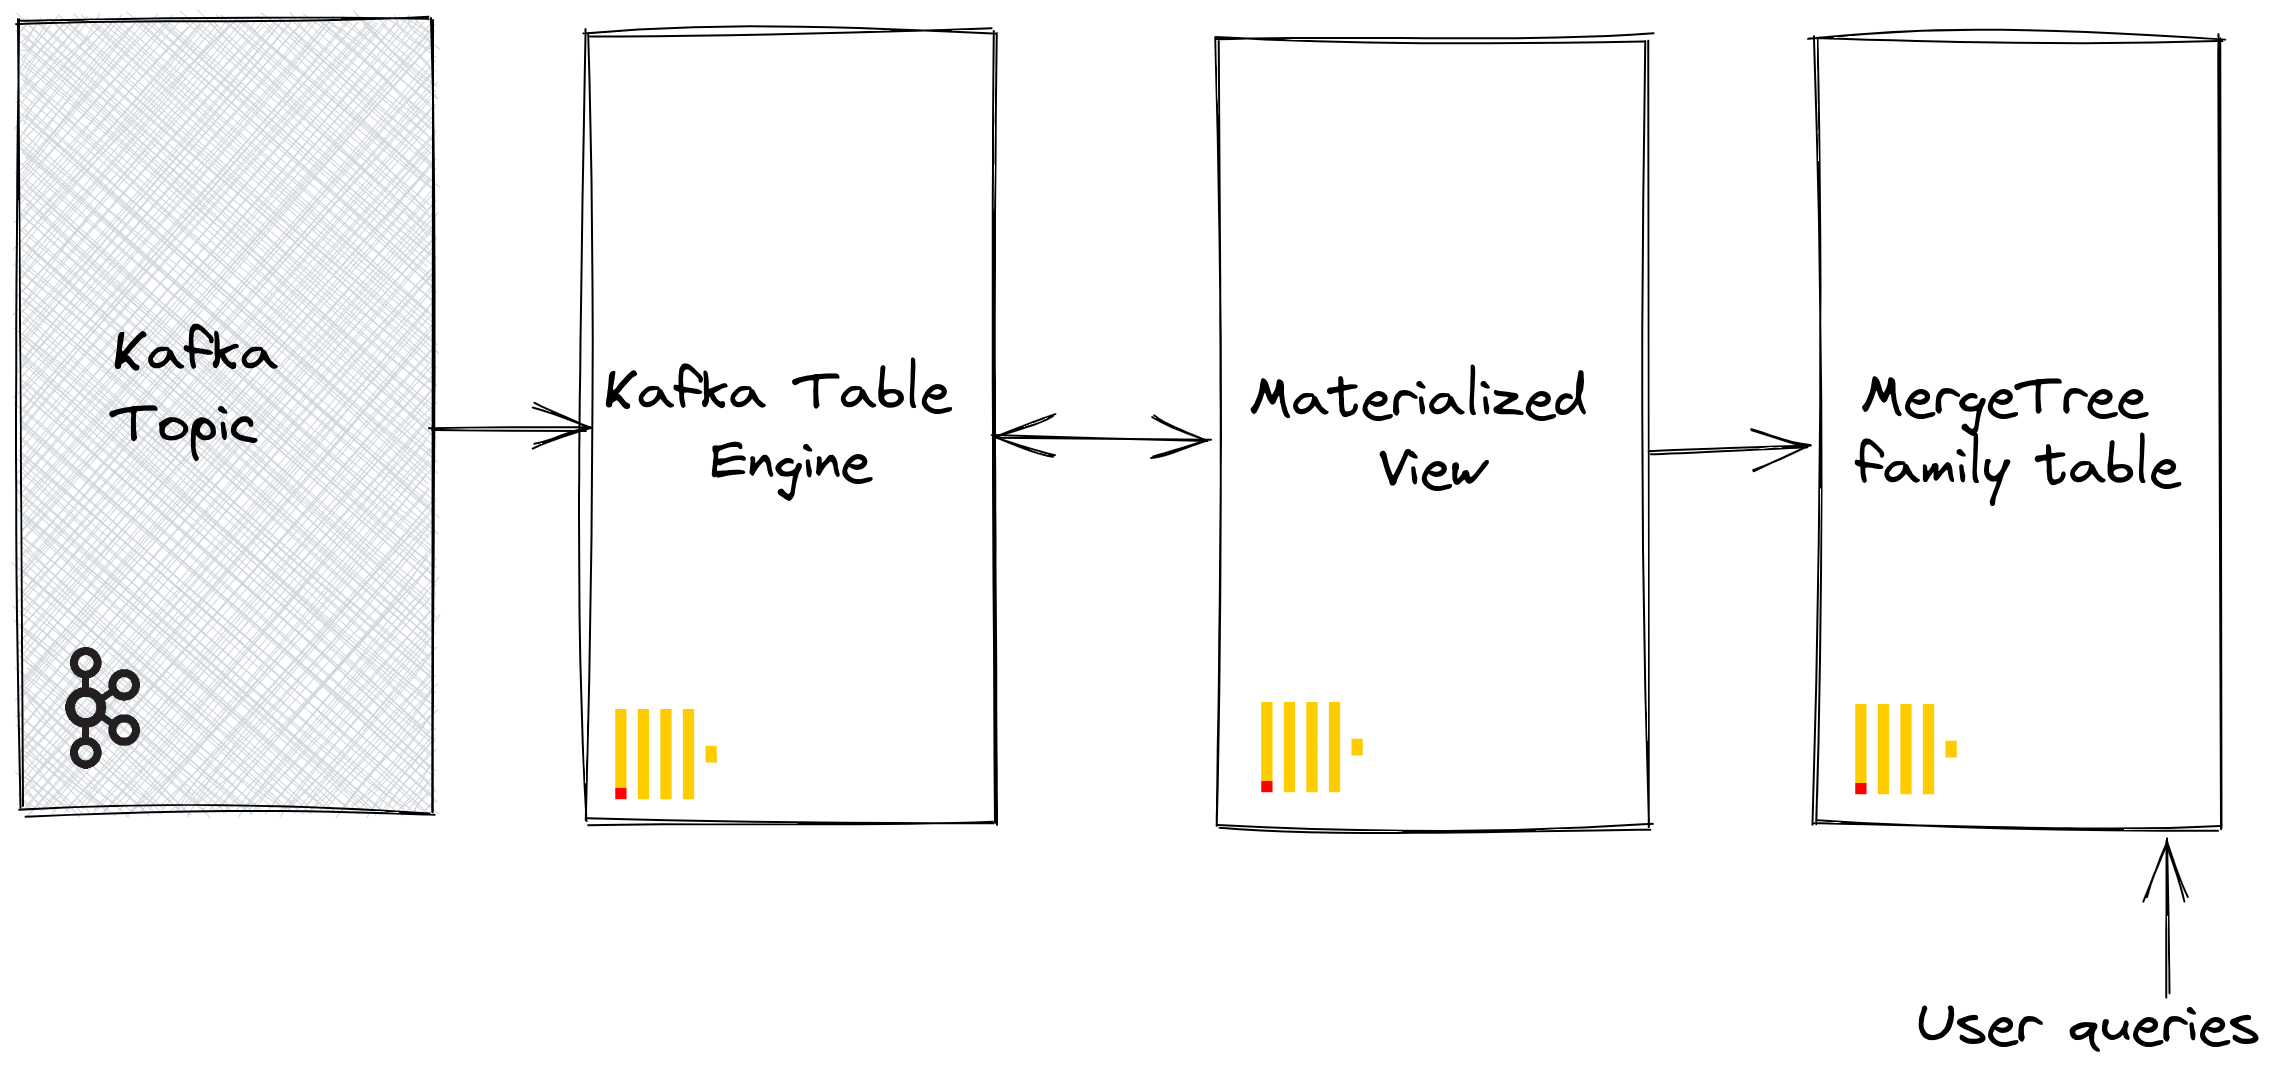
\includegraphics[width=.7\textwidth]{../Images/SpecificaTecnica/kafka_engine_architecture.png}
  \caption{Architettura di Kafka Engine in ClickHouse}
  \label{fig:Architettura_kafka_engine}
\end{figure}

\subsubsection{Trasferimento dati tramite Materialized View} \label{sec:materializedView}
Una materialized view funge da ponte tra la fonte dei dati (Kafka Engine) e la destinazione dei dati (MergeTree). Quando nuovi dati vengono scritti nella tabella Kafka Engine, la materialized view viene attivata automaticamente.\\
La materialized view esegue una query sulla tabella Kafka Engine per selezionare i dati più recenti. Una volta selezionati, questi dati vengono inseriti nella tabella di destinazione (ad esempio, una tabella MergeTree). Questo processo avviene in modo automatico e immediato, senza bisogno di intervento manuale.\\
In pratica, la materialized view si assicura che la tabella di destinazione sia sempre aggiornata con i dati più recenti presenti nella tabella Kafka Engine. Questo offre numerosi vantaggi:
\begin{itemize}
  \item \textbf{Automatizzazione del processo}: Non è necessario eseguire manualmente operazioni di trasferimento dati da una tabella all'altra. La materialized view si occupa di tutto in modo automatico;
  \item \textbf{Efficienza}: Il trasferimento dei dati avviene in tempo reale, garantendo che la tabella di destinazione sia sempre allineata con la fonte dei dati senza ritardi;
  \item \textbf{Ottimizzazione delle risorse}: Il processo di trasferimento dei dati è gestito in modo efficiente, utilizzando al meglio le risorse disponibili e garantendo prestazioni elevate.
\end{itemize}
Nel contesto specifico, le materialized view sono responsabili di eseguire controlli sui dati, come ad esempio la verifica della loro correttezza ed affidabilità nel contesto di utilizzo, prima di inserirli nella tabella di destinazione. Questo processo assicura che i dati siano sempre affidabili e pronti per l'analisi, senza la necessità di ulteriori operazioni di pulizia o preparazione.\\
Per esempio, nel caso dei dati di umidità raccolti da sensori in un'area urbana, la materialized view potrebbe eseguire controlli per assicurarsi che i valori rientrino all'interno di un intervallo plausibile e che non ci siano discrepanze improbabili. Ciò garantirebbe che i dati di umidità inseriti nella tabella di destinazione siano accurati e affidabili per l'analisi meteorologica o ambientale.


\subsubsection{Tabella di origine di Kafka Engine per un sensore generico}
Le tabelle del database impiegate per registrare le misurazioni di ciascuna tipologia di sensore presentano una configurazione sostanzialmente simile, differenziandosi principalmente per il tipo di dato della colonna relativa alla misurazione e per il \textit{topic} di riferimento utilizzato per ottenere le misurazioni.
Nello specifico per ogni sensore si avrà la seguente tabella Clickhouse:
\begin{figure}[H]
    \centering
    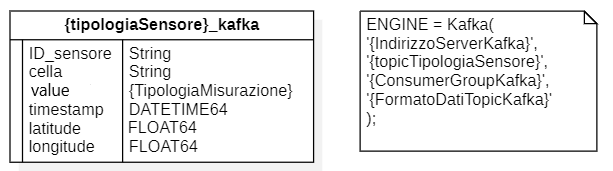
\includegraphics[width=.6\textwidth]{../Images/SpecificaTecnica/sensorType_kafka.PNG}
    \caption{Tabella sensore generico per il reperimento da kafka - ClickHouse}
    \label{fig:Reperimento_kafka_clickhouse}
  \end{figure}

    La tabella è configurata con il motore di storage \textit{Kafka}, il che significa che i dati verranno letti da un \textit{topic Kafka}. 

    I campi sono:
    \begin{itemize}
        \item \textbf{ID\_sensore}: un campo di tipo \textit{String} che identifica univocamente il sensore che ha effettuato la misurazione;
        \item \textbf{cella}: un campo di tipo \textit{String} che rappresenta la cella della città in cui è stata effettuata la misurazione;
        \item \textbf{value}: un campo di tipo variabile a seconda del tipo di misurazione che contiene il valore della temperatura;
        \item \textbf{timestamp}: campo di tipo \textit{DATETIME64} che rappresenta il timestamp della misurazione della temperatura;
        \item \textbf{latitude}: un campo di tipo \textit{Float64} che rappresenta la latitudine del luogo dove è stata effettuata la misurazione;
        \item \textbf{longitude}: un campo di tipo \textit{Float64} che rappresenta la longitudine del luogo dove è stata effettuata la misurazione.
    \end{itemize}

    Mentre i parametri esposti racchiusi da parentesi graffe variano per ogni tipolgia di sensore correlato alla misurazione e sono:
    \begin{itemize}
        \item \textbf{tipologiaSensore}: viene sostituito con la tipologia del sensore che effettua le misurazioni salvate nella tabella; (ex. temperatures)
        \item \textbf{TipoDatoMisurazione}: viene sostituito con il tipo del dato che rappresenta la misurazione (ex. Float32, UInt8);
        \item \textbf{IndirizzoServerKafka}: specifica l'indirizzo del server Kafka.
        Nel nostro caso il server Kafka è in esecuzione su un container \textit{Docker} raggiungibile tramite l'indirizzo:
         \textit{'kafka:9092'};
        \item \textbf{topicTipologiaSensore}: specifica il nome del topic Kafka da cui leggere i dati (ex.temperature);
        \item \textbf{ConsumerGroupKafka}: specifica il nome del consumer group Kafka che verrà utilizzato per leggere i messaggi dal topic \textit{Kafka} denominato 'temperature'.
        Un consumer group in \textit{Kafka} è un gruppo di consumatori che lavorano insieme per consumare i messaggi da uno o più topic. Ogni messaggio inviato a un \textit{topic Kafka} può essere consumato da uno dei consumatori nel gruppo. I consumer all'interno di uno stesso gruppo condividono l'elaborazione dei messaggi all'interno dei topic: ogni messaggio viene elaborato da uno e un solo consumatore all'interno del gruppo. Nel nostro caso sarà sempre '\textit{CG\_Clickhouse\_1}' per indicare il servizio di salvataggio \textit{Clickhouse}.
        \item \textbf{FormatoDatiTopicKafka}: specifica il formato dei dati nel \textit{topic Kafka}. Nel nostro caso, i dati sono nel formato JSONEachRow, che è un formato di serializzazione JSON di \textit{ClickHouse} che consente di scrivere o leggere record JSON separati da una riga. Quindi avremo che <<FormatoDatiTopicKafka>> = JSONEachRow.
        \item \textbf{KafkaSkipBrokenMessages}: specifica il numero di errori da tollerare durante il parsing dei messaggi, configurato a livello di tabella, rappresenta la quantità massima di errori accettabili che il sistema può gestire durante il processo di analisi dei messaggi. Questo parametro consente di regolare il livello di tolleranza agli errori a livello di tabella, offrendo la possibilità di controllare quanto il sistema debba essere flessibile nell'interpretazione dei dati.
    \end{itemize}

    
    \subsubsection{Misurazioni temperatura} \label{sec:tab_temperatures}
    Di seguito viene presentata una configurazione dettagliata per l'archiviazione delle misurazioni di temperatura. Tale configurazione si applica alla tabella 'temperatures\_kafka', progettata per acquisire dati da un topic Kafka. La tabella è strutturata per includere l'ID del sensore (String), la posizione della cella (String), il valore della temperatura misurato (Float32), il timestamp della misurazione (DATETIME64), la latitudine (Float64) e la longitudine (Float64) del sensore. Ogni campo è definito con un tipo di dato specifico al fine di garantire la precisione e l'integrità dei dati.
    
    \begin{figure}[H]
        \centering
        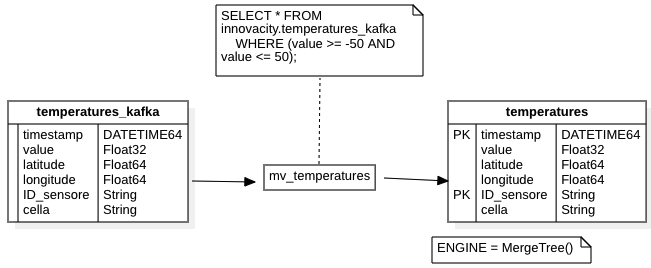
\includegraphics[width=1\textwidth]{../Images/SpecificaTecnica/temperatures.png}
        \caption{Tabella temperatures\_kafka e temperatures}
        \label{fig:temperatures}
      \end{figure}
    
    La tabella 'temperatures\_kafka' è essenziale nel contesto dell'architettura dei dati, poiché funge da tramite tra un topic Kafka e il sistema di gestione dei dati ClickHouse. Questa tabella agisce come un'interfaccia di origine, trasformando i flussi di dati provenienti dal topic Kafka in un formato comprensibile per ClickHouse. Successivamente, una Materialized View, in questo caso 'mv\_temperatures', opera su questa tabella per trasferire i dati ottenuti verso la tabella di destinazione 'temperatures' come spiegato in \ref{sec:materializedView}.
    
    \paragraph{Projections per misurazioni di temperatura} \label{sec:temp_projections}
    Durante la fase di progettazione, è stata dedicata particolare attenzione all'utilizzo delle tabelle precedentemente descritte e alle richieste che verranno formulate su di esse. È emerso che, considerando il requisito di suddividere la città in una serie di celle e specificare la cella di origine della misurazione, la filtrazione delle misurazioni per celle diventerà una richiesta frequente al database. Di conseguenza, si è optato per l'utilizzo delle PROJECTIONS, le quali sono dettagliatamente descritte nella sezione \ref{sec:projections}.
    \vspace{0,3cm}
    \begin{lstlisting}[caption={Esempio di proiezione e materializzazione in una tabella}, captionpos=b]
      --Projection per tabella temperatures
      ALTER TABLE innovacity.temperatures ADD PROJECTION tmp_sensor_cell_projection (SELECT * ORDER BY cella);
      ALTER TABLE innovacity.temperatures MATERIALIZE PROJECTION tmp_sensor_cell_projection;
  \end{lstlisting}
    \vspace{0,3cm}
    La proiezione ci consentirà di effettuare rapidamente filtraggi basati sulle celle, anche se tale attributo non è definito come \textit{PRIMARY\_KEY} nella tabella originale.

\subsubsection{Misurazioni umidità}
Le considerazioni relative al salvataggio delle misurazioni di umidità coincidono con quelle espresse nella sezione \ref{sec:temp_projections} riguardo alle misurazioni di temperatura.
In questa situazione, dove le misure riguardano l’umidità, la tabella di destinazione ClickHouse è nominata ‘humidity’:

\begin{figure}[H]
    \centering
    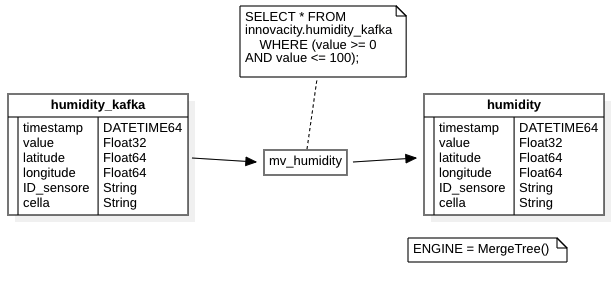
\includegraphics[width=1\textwidth]{../Images/SpecificaTecnica/humidity.png}
    \caption{Tabella humidity\_kafka e humidity}
    \label{fig:humidity_tables}
  \end{figure}

\paragraph{Projections per misurazioni di umidità} 
Dopo aver considerato le stesse argomentazioni presentate nella sezione \ref{sec:tab_temperatures} riguardanti le misurazioni di temperatura, abbiamo deciso di estendere l'utilizzo delle PROJECTION anche alle misurazioni di umidità. I vantaggi ottenuti risultano essere simili a quelli evidenziati per le misurazioni di temperatura, come descritto nella stessa sezione. A seguire, vengono illustrate le configurazioni delle PROJECTION relative alle tabelle delle misurazioni di umidità:

\begin{lstlisting}
    --Projection per tabella humidity
    ALTER TABLE innovacity.humidity ADD PROJECTION umd_sensor_cell_projection (SELECT * ORDER BY cella);
    ALTER TABLE innovacity.humidity MATERIALIZE PROJECTION umd_sensor_cell_projection;
\end{lstlisting}


\subsubsection{Misurazioni di polveri sottili}Le considerazioni concernenti l'archiviazione delle misurazioni di polveri sottili corrispondono a quelle espresse nella sezione \ref{sec:temp_projections} in merito alle misurazioni di temperatura.

\begin{figure}[H]
    \centering
    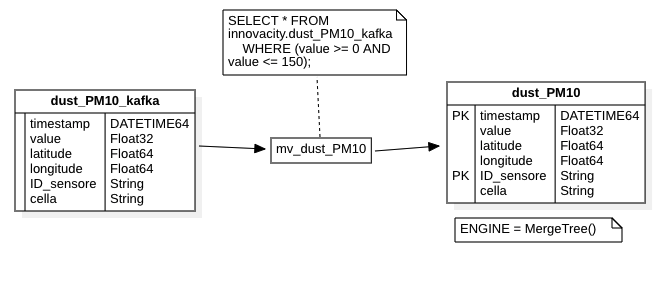
\includegraphics[width=1\textwidth]{../Images/SpecificaTecnica/dust_PM10.png}
    \caption{Tabella dustPM10\_kafka e dustPM10}
    \label{fig:dust_table}
  \end{figure}

\paragraph{Projections per misurazioni di polveri sottili} 
Dopo aver considerato le stesse argomentazioni presentate nella sezione \ref{sec:tab_temperatures} riguardanti le misurazioni di temperatura, abbiamo deciso di estendere l'utilizzo delle PROJECTION anche alle misurazioni di polveri sottili. I vantaggi ottenuti risultano essere simili a quelli evidenziati per le misurazioni di temperatura, come descritto nella stessa sezione. A seguire, vengono illustrate le configurazioni delle PROJECTION relative alle tabelle delle misurazioni di polveri sottili:

\begin{lstlisting}
  --Projection per tabella dust_PM10
  ALTER TABLE innovacity.dust_PM10 ADD PROJECTION dust_sensor_cell_projection (SELECT * ORDER BY cella);
  ALTER TABLE innovacity.dust_PM10 MATERIALIZE PROJECTION dust_sensor_cell_projection;
\end{lstlisting}

\subsubsection{Misurazioni guasti elettrici} \label{sec:tab_guasti}
Segue una dettagliata configurazione per l'archiviazione delle misurazioni relative ai guasti elettrici, applicabile alla tabella 'electricalFault\_kafka' progettata per acquisire dati dal topic Kafka. La struttura della tabella include l'ID del sensore (String), la posizione della cella (String), il valore misurato (UInt8), il timestamp della misurazione (DATETIME64), la latitudine (Float64) e la longitudine (Float64) del sensore, ciascuno definito con un tipo di dato specifico per garantire la precisione e l'integrità dei dati.

\begin{figure}[H]
    \centering
    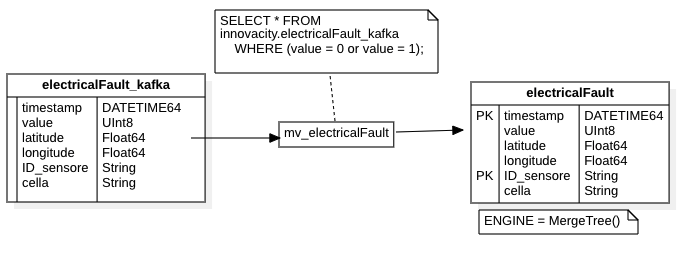
\includegraphics[width=1\textwidth]{../Images/SpecificaTecnica/electricalFault.png}
    \caption{Tabella electricalFault\_kafka e electricalFault}
    \label{fig:electricalFault_tables}
  \end{figure}

Le considerazioni concernenti l'archiviazione delle misurazioni di guasti elettrici corrispondono a quelle espresse nella sezione \ref{sec:temp_projections} in merito alle misurazioni di temperatura.

\paragraph{Projections per misurazioni di guasti elettrici} 
Dopo aver considerato le stesse argomentazioni presentate nella sezione \ref{sec:tab_temperatures} riguardanti le misurazioni di temperatura, abbiamo deciso di estendere l'utilizzo delle PROJECTION anche alle misurazioni di guasti elettrici. I vantaggi ottenuti risultano essere simili a quelli evidenziati per le misurazioni di temperatura, come descritto nella stessa sezione. A seguire, vengono illustrate le configurazioni delle PROJECTION relative alle tabelle delle misurazioni di guasti elettrici:

\begin{lstlisting}
  --Projection per tabella electricalFault
  ALTER TABLE innovacity.electricalFault ADD PROJECTION elctF_sensor_cell_projection (SELECT * ORDER BY cella);
  ALTER TABLE innovacity.electricalFault MATERIALIZE PROJECTION elctF_sensor_cell_projection;
\end{lstlisting}

\subsubsection{Misurazioni stazioni di ricarica} Le considerazioni concernenti l'archiviazione delle misurazioni delle stazioni di ricarica corrispondono a quelle espresse nella sezione \ref{sec:tab_guasti} in merito alle misurazioni guasti elettrici.

\begin{figure}[H]
    \centering
    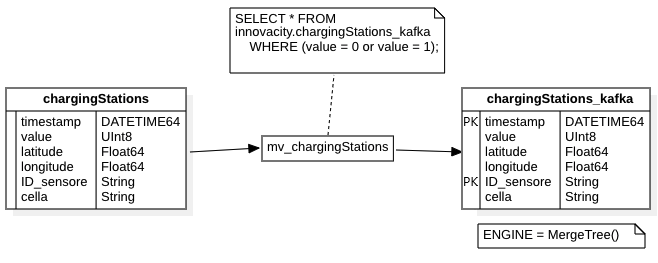
\includegraphics[width=1\textwidth]{../Images/SpecificaTecnica/chargingStations.png}
    \caption{Tabella chargingStation\_kafka e chargingStation}
    \label{fig:chargingStation_tables}
  \end{figure}

\paragraph{Projections per misurazioni delle stazioni di ricarica}
Dopo aver considerato le stesse argomentazioni presentate nella sezione \ref{sec:tab_temperatures} riguardanti le misurazioni di temperatura, abbiamo deciso di estendere l'utilizzo delle PROJECTION anche alle misurazioni delle stazioni di ricarica. I vantaggi ottenuti risultano essere simili a quelli evidenziati per le misurazioni di temperatura, come descritto nella stessa sezione. A seguire, vengono illustrate le configurazioni delle PROJECTION relative alle tabelle delle misurazioni delle stazioni di ricarica:

\begin{lstlisting}
  --Projection per tabella chargingStations
  ALTER TABLE innovacity.chargingStations ADD PROJECTION chS_sensor_cell_projection (SELECT * ORDER BY cella);
  ALTER TABLE innovacity.chargingStations MATERIALIZE PROJECTION chS_sensor_cell_projection;
\end{lstlisting}

\subsubsection{Misurazioni isole ecologiche}
Le considerazioni concernenti l'archiviazione delle misurazioni delle isole ecologiche corrispondono a quelle espresse nella sezione \ref{sec:tab_temperatures} in merito alle misurazioni di temperatura.

\begin{figure}[H]
  \centering
  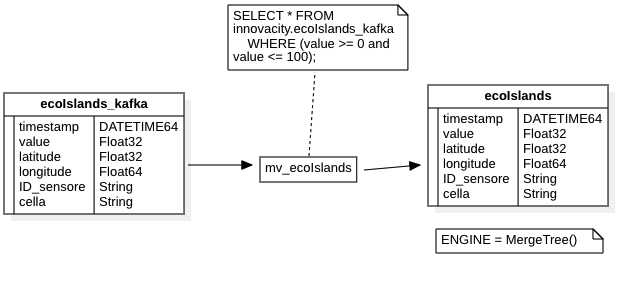
\includegraphics[width=1\textwidth]{../Images/SpecificaTecnica/ecoIslands.png}
  \caption{Tabella ecoIslands\_kafka e ecoIslands}
  \label{fig:ecoIslands_tables}
\end{figure}

\paragraph{Projections per misurazioni delle isole ecologiche} 
Dopo aver considerato le stesse argomentazioni presentate nella sezione \ref{sec:tab_temperatures} riguardanti le misurazioni di temperatura, abbiamo deciso di estendere l'utilizzo delle PROJECTION anche alle misurazioni delle isole ecologiche. I vantaggi ottenuti risultano essere simili a quelli evidenziati per le misurazioni di temperatura, come descritto nella stessa sezione. A seguire, vengono illustrate le configurazioni delle PROJECTION relative alle tabelle delle misurazioni delle isole ecologiche:

\begin{lstlisting}
  --Projection per tabella ecoIslands
  ALTER TABLE innovacity.ecoIslands ADD PROJECTION umd_sensor_cell_projection (SELECT * ORDER BY cella);
  ALTER TABLE innovacity.ecoIslands MATERIALIZE PROJECTION umd_sensor_cell_projection;
\end{lstlisting}

\subsubsection{Misurazioni sensori livello dell’acqua}
Le considerazioni concernenti l'archiviazione delle misurazioni dei sensori di livello dell'acqua corrispondono a quelle espresse nella sezione \ref{sec:tab_guasti} in merito alle misurazioni guasti elettrici.

\begin{figure}[H]
  \centering
  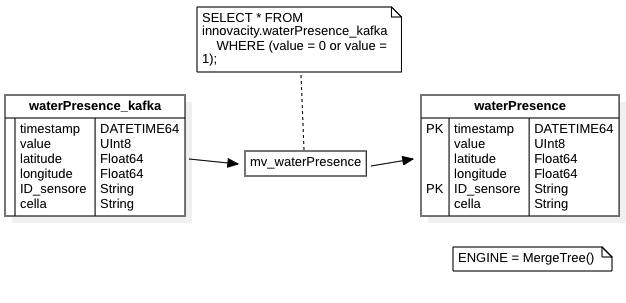
\includegraphics[width=1\textwidth]{../Images/SpecificaTecnica/waterPresence.png}
  \caption{Tabella waterPresence\_kafka e waterPresence}
  \label{fig:waterPresence_tables}
\end{figure}

\paragraph{Projections per misurazioni del livello dell'acqua} 
Dopo aver considerato le stesse argomentazioni presentate nella sezione \ref{sec:tab_temperatures} riguardanti le misurazioni di temperatura, abbiamo deciso di estendere l'utilizzo delle PROJECTION anche alle misurazioni del livello d'acqua. I vantaggi ottenuti risultano essere simili a quelli evidenziati per le misurazioni di temperatura, come descritto nella stessa sezione. A seguire, vengono illustrate le configurazioni delle PROJECTION relative alle tabelle delle misurazioni del livello d'acqua:
\begin{lstlisting}
  --Projection per tabella waterPresence
  ALTER TABLE innovacity.waterPresence ADD PROJECTION waPr_sensor_cell_projection (SELECT * ORDER BY cella);
  ALTER TABLE innovacity.waterPresence MATERIALIZE PROJECTION waPr_sensor_cell_projection;
\end{lstlisting}